\documentclass[12pt]{CPP}
\usepackage{fancyhdr}
\usepackage{graphicx}
\usepackage{subfigure}
\usepackage{listings}
\usepackage{mathtools}
\usepackage{longtable}
\usepackage{hyphenat}
\usepackage{caption}

\usepackage[round, sort]{natbib}
\bibliographystyle{turabian}
\setlength{\bibhang}{.3in}
\bibpunct{[}{]}{,}{a}{}{,}

\begin{document}

    \titleone{Dithered Index}
    \titletwo{}
    \doctype{Project}
    \doctypeUp{Project}
    \degree{Master of Science}
    \field{Computer Science}
    \Author{Diana Arrieta}
    \Advisor{Amar Raheja}
    \MemberA{Robert Kerbs}
    \MemberB{Committee Member 2}
    \Year{2013}
    \quarter{Summer}

\Abstract{
Textures are commonly used for everyday graphics implementations, such as modeling, rendering and display. As the bandwidth of hardware maintains its current rate of improvement, random access memory and speed continue to outpace these improvements, creating a bottle neck for accessing subsequent information that is needed for the next operations. Improving textures by making them smaller to push through the pipeline, or able to access more in a single operation would be able to overcome bandwidth limitations.}

\Acknowledgments{
\begin{center}
My Mom, who always pushed and believed in me.
\end{center}
}

\coversheet
\titlepage
\signaturepage
\acknowledgmentspage
\abstractpage
\newpage

\tableofcontents
\newpage
\listoffigures
\newpage
\listoftables
\newpage

\pagenumbering{arabic} \setcounter{page}{1}
\section{Introduction}

\subsection{Texture Compression}
Compared to compression of every type of image, texture compression focuses on compressing a specific type of images that are used in graphics processing. While most of the methods used in other compression algorithms can apply to images without modification, texture based methods have the restrictions that random access be available to individual textels and decompression completes in a reasonable amount of time.

\subsection{Motivation}
When computers and hand-held devices are assembled, either in an assembly line or as a do-it-yourself project by an ambitious user, if the use of a screen such as an LCD display is needed, the device will often requires the use of a graphics processor, integrated into the motherboard or discrete as a graphics card. These graphics cards are often a computer in their own right, having a multitude of cores, a supply of their own Random Access Memory (RAM), and even a cooling system. Whether if the graphics is integrated or discrete, each of these various types of graphics processors support some form of graphics rendering, decoding and display. Most of these graphics processors have been developed to support the current de facto standard of the Microsoft DirectX application programming interface (API) to handle multimedia such as calculations for algorithms used by gaming engines, rendering, and video decoding. For operating systems that don't support proprietary drivers, such as those that come from nVidia or ATI, open source drivers are available under another standard called OpenGL that can support most modern day video cards. Hand held devices such as smart phones and gaming devices also come with graphics processors that support programming in a different version of OpenGL called OpenGL for Embedded Systems (OpenGL ES).

As technology improves, graphics processing also improves along with it, becoming increasingly detailed and smooth. Unfortunately, to improve the visual appearance of the final rendered products, larger and more detailed textures have to be used. Image compression has helped in improving storage of large amounts of data in both lossy and lossless formats. Compression works by removing redundancies that are frequent in raw image data, resulting in files that take up a fraction of the space they would otherwise occupy in their raw format.

\subsection{Applications}
Reducing texture storage has many graphics applications which can benefit from a method that can lower the rate at which colors become lost due to transformation and lossy compression. Often, algorithms that perform texture compression can have statistics which can be used to determine whether the targeted block should be compressed to a lesser extent, or at all, if the resulting noise to signal ratio is not within an acceptable range.

\newpage
\section{Literature Review}

\subsection{Human Vision}

\subsubsection{The Human Eye}
The human eye contains several structures that enables people to see human visual perception. The cornea and sclera protect the delicate inner structures of the eye, while the choroid provides nutrition through blood vessels throughout the eye. The muscles in the iris control the amount of light that enters the eye through the pupil, and so contracts in bright light, and dilates when there is a lack of lighting. Underneath the iris lies the lens. The lens has it's own muscle that changes it's size. By changing it's size, light can be focused properly on the retina. The retina processes the light it receives into signals that are transmitted via the optic nerve, and the image is reconstructed by the brain.

\begin{figure}[!htbp]
\begin{center}
\subfigure{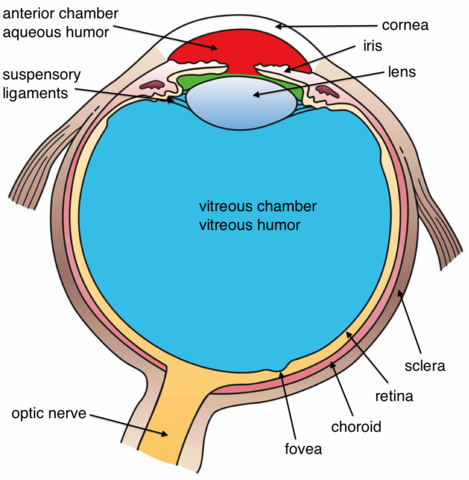
\includegraphics[scale=1]{./images/diagrams/eye_structures}}
\caption{Diagram of structures within the human eye.}
\end{center}
\end{figure}

The retina contains 75 to 150 million rods that process overall illumination, and as such don't provide color information. In fact, the wide distribution of rods causes several rods to share a single nerve, so objects lack detail when seen in dim lighting. Cones have a narrower distribution, being concentrated at the central area of the retina called the fovea. Cones are highly sensitive to color in bright light. Each cone has it's own nerve connection, and so objects have a greater amount of detail. \citep{Rafael}

\begin{figure}[!htbp]
\begin{center}
\subfigure{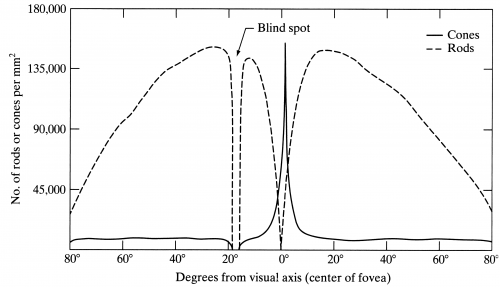
\includegraphics[scale=0.75]{./images/diagrams/rods_cones}}
\caption{The distribution of rods and cones along the retina. Note the gap which is where the optic nerve would emerge.}
\end{center}
\end{figure}

\subsubsection{Tolerance and MacAdam Ellipses}
The human eye can perceive about 10 million different colors. True color, also known as 24-bit color, uses 8 bits to represent each red, green, and blue component, allowing 256 different shades for each. All together, true color can display up to 16,777,216 different colors.

Color vision has a tendency to be subjective to different lighting and surroundings. By knowing how the human eye perceives color and visual details, slight adjustments can be made for a given color value without any detection or loss of visual information. \citep{MacAdam}

\begin{figure}[!htbp]
\begin{center}
\subfigure{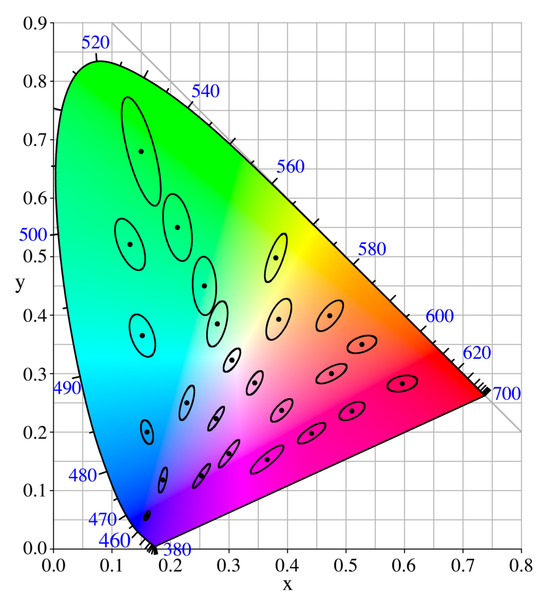
\includegraphics[scale=0.35]{./images/diagrams/macadam}}
\caption{MacAdam ellipses shown ten times their actual size on the CIE 1931 XYZ color space. Colors inside an ellipse visually match the color in the center.}
\end{center}
\end{figure}

\subsubsection{Dithering}
When lowering the number of bits per channel used in a pixel, an often used method is simply rounding the component to the nearest number. While this process is easy to use, it also results in banding in an image. By using a number of dithering algorithms, a predetermined palette is selected and colors are replaced with their closest match using heuristics. As colors are swapped out, error can be accumulated into the surrounding pixels, allowing a different color to be used when there is not a suitable match for an existing one, causing mixed patterns.

\begin{figure}[!htbp]
\begin{center}
\subfigure{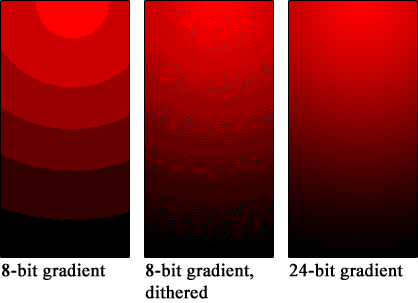
\includegraphics[scale=0.6]{./images/compress/banding_gradient}}
\caption{Banding in a gradient. Banding is reduced when dithering is applied.}
\end{center}
\end{figure}

\begin{figure}[!hbp]
\begin{center}
\subfigure{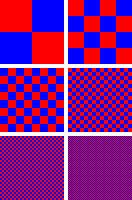
\includegraphics[scale=1]{./images/compress/dithering}}
\subfigure{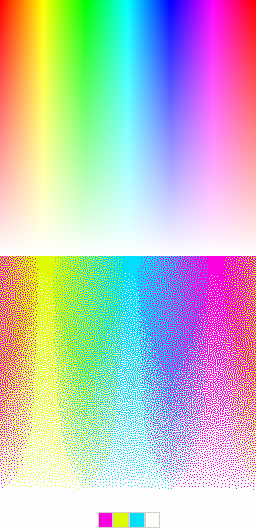
\includegraphics[scale=0.38]{./images/compress/rainbow_dithering}}
\caption{Using dithering, more colors can be represented using a reduced color palette.}
\end{center}
\end{figure}

In physical media, it is not uncommon to encounter half-toning. Halftones only use one color, and distribute varying sizes of dots to create the illusion of different tones. Dithering allows the use different colors placed such that it seems that there are more colors than actually available in the reduced palette. \citep{Knuth}

\subsection{Compression}

\subsubsection{Defining Compression}
Compression involves encoding information into fewer bits than would be occupied by the original. There are two types of compression currently in use. Lossless analyzes the input and identifies redundancies that can be represented in fewer bits. Using this method, no information is lost, and it is ideal for compressing text based files and images. Lossy compression instead removes finer details completely, which can be tuned according to what is acceptable for images and video.

\subsubsection{Entropy}
Entropy is defined as a measure of uncertainty given a random variable.

Shannon's theorem states such that it is impossible to compress data in a lossless form such that the average number of bits per symbol used is less than what was used in the source. As such, when fewer symbols are used to represent the compressed data, the resulting compressed information is considered to be a lossy format. \citep{Shannon}

\[
H(X) = -\sum_{i=1}^{n} p(x_i)log_b p(x_i)
\]

\subsection{Lossless Compression}
Lossless compression is most commonly used when any loss of information that would cause the target data to become meaningless if any part of it would be lost or if the user would prefer if all the data in an image be preserved. Lossless has the inherent problem that if a file has minimal redundancy to remove or is not large enough to detect eventual redundant information, the file may not compress at all, or it may even grow in size and occupying more space to accommodate compression information.

\subsubsection{Huffman Coding}
Huffman coding is an entropy encoder. Given an input, the algorithm will count each occurrence of every character encountered. With this, the frequency is calculated for each character and added to a frequency table. Using the table, a binary tree is constructed, giving characters with a higher frequency a shorter code representing it, and less frequent characters a longer code. These trees can also be constructed using pre-calculated frequencies for a particular subject matter.

\renewcommand{\arraystretch}{.8}
\setlength{\tabcolsep}{6pt}
\begin{center}
\begin{figure}[!htbp]
\begin{tabular}{| l | l | l | l | l | l | l | l |}
\hline
Letter & Frequency & Letter & Frequency & Letter & Frequency & Letter & Frequency \\ \hline
e & 0.12702 & h & 0.06094 & w & 0.02360 & k & 0.00772 \\ \hline
t & 0.09056 & r & 0.05987 & f & 0.02228 & j & 0.00153 \\ \hline
a & 0.08167 & d & 0.04253 & g & 0.02015 & x & 0.00150 \\ \hline
o & 0.07507 & l & 0.04025 & y & 0.01974 & q & 0.00095 \\ \hline
i & 0.06966 & c & 0.02782 & p & 0.01929 & z & 0.00074 \\ \hline
n & 0.06749 & u & 0.02758 & b & 0.01492 &   &         \\ \hline
s & 0.06327 & m & 0.02406 & v & 0.00978 &   &         \\ \hline
\end{tabular}
\caption{Frequency for common letters in the English language.}
\end{figure}
\end{center}

\begin{figure}[!htbp]
\begin{center}
\subfigure{\includegraphics[scale=1.4]{./images/diagrams/Morse}}
\caption{A Huffman binary tree. This is the tree also used for Morse code.}
\end{center}
\end{figure}

\subsubsection{Lempel-Ziv-Welch} Lempel-Ziv-Welch and it's variants compress data using a dictionary coder, or substitution coder. As the algorithm encounters patterns that it has seen before, it substitutes these with a shorter representation provided that it is already in the dictionary. If not, it creates one on the spot and outputs the corresponding code. Dictionary algorithms work best on longer streams of input, as this allows the dictionary to accumulate entries and create longer strings. The Lempel-Ziv-Welch algorithm has the added benefit that the dictionary does not have to be stored with the compressed result, as it is reconstructed as it reads the file. \citep{Ziv}

\begin{quote}
\begin{figure}[!htbp]
\vspace{-20pt}
\begin{verbatim}
w = NIL;
   while ( read a character k )
   {
      if wk exists in the dictionary
         w = wk;
      else
         add wk to the dictionary;
      output the code for w;
      w = k;
   }
\end{verbatim}
\vspace{-20pt}
\caption{Pseudo-code for LZW (compression).}
\end{figure}
\end{quote}

\begin{quote}
\begin{figure}[!htbp]
\begin{verbatim}
read a character k;
   output k;
   w = k;
   while ( read a character k )
   /* k could be a character or a code. */
   {
      if k exists in the dictionary
         entry = dictionary entry for k;
         output entry;
         add w + entry[0] to dictionary;
         w = entry;
      else
         output entry = w + firstCharacterOf(w);
      add entry to dictionary;
      w = entry;
   }
\end{verbatim}
\vspace{-20pt}
\caption{Pseudo-code for LZW (decompression).}
\vspace{-20pt}
\end{figure}
\end{quote}

\subsection{Lossy Compression}
Lossy compression is used when loss of information is acceptable to a certain level. Lossy compression algorithms can often be fine tuned to the users needs. If smaller file size is desired, the user can lower the quality of the resulting image to reach the target size. Because large amounts of information can be removed from the source data, file sizes for lossy compression can easily be smaller than their lossless counterparts. Since some information is thrown out, these methods are typically reserved for images, video and audio formats since loss of information is acceptable to achieve the desired result.

\subsubsection{Wavelet Transform}
Wavelets are a tool to process a variety of signals. These transforms can be used to remove noise and blurring, and also compress data, which are easily invertible. The simplest transform is called the Haar transform. A single eight point signal can be decomposed into four average signal values, and four being their difference. This can be performed again on the results calculated for average value as many as three times for an eight point signal. At the end, the coefficients for each set can be stored and used to reconstruct the image. This type of compression is actually used in the JPEG 2000 file type. \citep{Chui}

\begin{figure}[!htbp]
\begin{center}
\subfigure{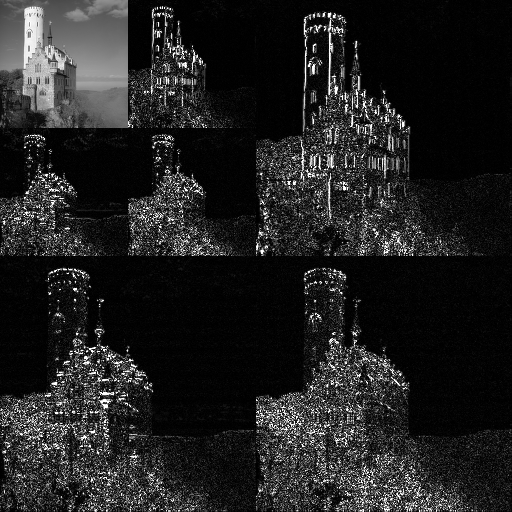
\includegraphics[scale=0.40]{./images/compress/wavelet}}
\subfigure{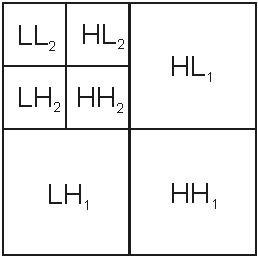
\includegraphics[scale=.8]{./images/compress/dia_wavelet}}
\caption{Image processed with a wavelet transform. Each block contains coefficients to reconstruct the original image.}
\end{center}
\end{figure}

\subsubsection{Motion Compensation (MPEG-2)}
Motion compensation is used in the MPEG-2 standard. It defines a picture that has been adjusted from a picture that was taken at a future point. In a movie, the most common reason the picture changes is because either the camera is moving or an object is moving within the frame. A frame that is created that contains the differences between the current frame and the next frame contains much more data if the camera has moved. By taking two frames and identifying the overlap from the camera panning, there is less data created, enabling a higher level of compression. MPEG-2 contains several frames to reconstruct the video stream. I frames contain initial data that are used to predict data in P (predicted) B (bi-directionally predicted) frames. These frames are often sent ahead of time so they can be generated in a timely fashion. \citep{Tudor}

\begin{figure}[!htbp]
\begin{center}
\subfigure{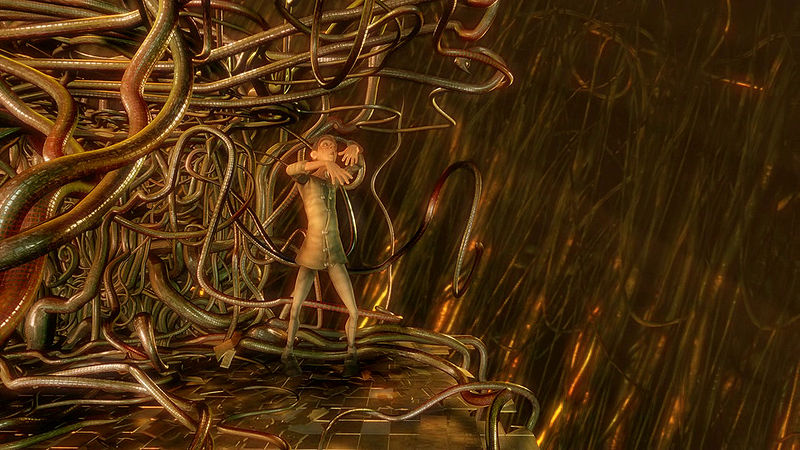
\includegraphics[scale=0.25]{./images/compress/original}}
\subfigure{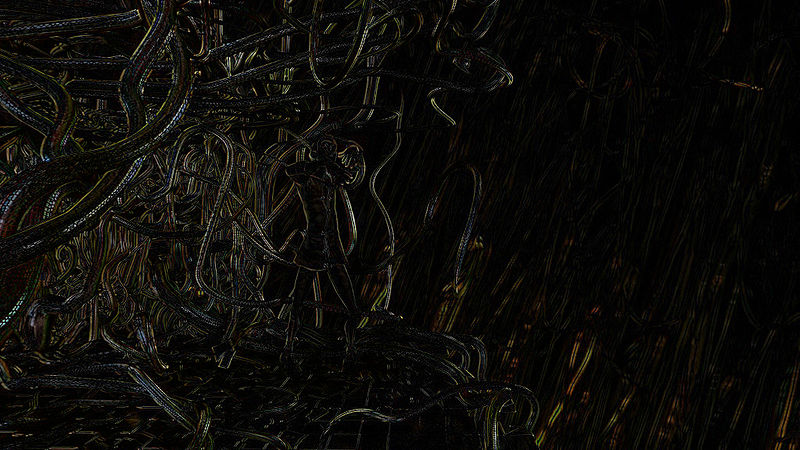
\includegraphics[scale=0.25]{./images/compress/difference}}
\subfigure{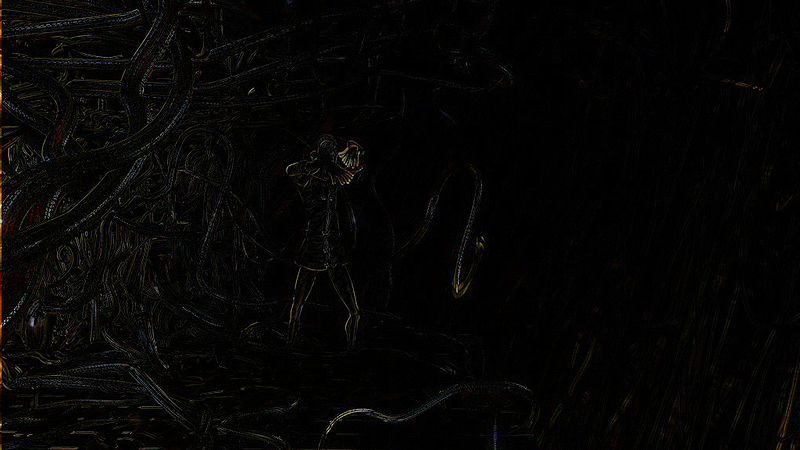
\includegraphics[scale=0.25]{./images/compress/motion}}
\caption{The original frame, the difference frame, and the motion compensated frame.}
\end{center}
\end{figure}

\subsection{Textures}
Textures typically are made up of images that are to be manipulated and mapped to a surface. This typically takes place the final step in the graphics pipeline and is performed by the texture mapping unit. Once all the objects are in place, textures are applied to the objects and the scene is finally rendered and shown on the output display. Textures can not only be used to contain color information, but also terrain information, lighting, and bump mapping in a different format. Textures that contain vector information are often not compressed as doing so would cause a loss of critical information that is used to calculate lighting information.

Textures can be optimized in various ways to enable graphics processors to access them and use them in an efficient manner. In a larger scale game, the number of textures can easily number into the hundreds, and finding a way to organize them so they can be found quickly can vary from the type of texture to what colors they mostly contain.

\subsubsection{Texture Storage Methods}
When saving textures for future use, they can be stored in various ways to save space on the hard drive and to enable more textures to be pushed through available bandwidth. While the most common way to have more textures available for the same amount of space is to compress the textures individually, there are various other methods to improve the rate at which they are read, and how many textures the designer would have to make.

\subsubsection{Atlas}
To decrease the number of reads required to have all the textures readily accessible in memory, textures are often bunched together into a single large file called a texture atlas. When these are created, they can either be done by hand or by a texture design software that can often be provided by the maker of the graphics processor. Texture packing has a different problem in that they must be packed carefully enough so as to make use of all the space in the atlas possible as they often have specific size requirements. Because of the nature of texture compression algorithms, textures that differ in color greatly should be arranged differently to avoid color bleeding into another texture. Textures that have different alpha channel requirements should be put into a different atlas altogether. A texture atlas is particularly efficient in that an entire scene can use up a single atlas, and the next scene can be rendered with another, keeping reads to hard disk or system memory to a minimum. \citep{Sherrod2008}

\begin{figure}[!htbp]
\begin{center}
\subfigure{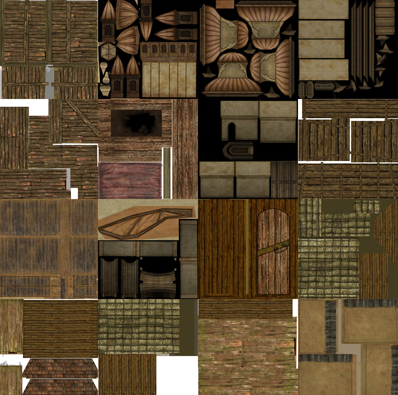
\includegraphics[scale=0.6]{./images/textures/texture_atlas}}
\caption{An atlas containing various textures for wooden objects such as doors, crates, flooring and walls.}
\end{center}
\end{figure}

\subsubsection{Synthesis}
Texture synthesis is a different way to render entire floors, walls and ceiling with a single texture that does not necessarily cover the entire space. By creating tile-able textures, a single texture can be used to cover surfaces without taking up the same amount of storage required of a larger texture. A common issue with tile-able textures is the lack of randomness in the surface which can be apparent in usually rich environments. Computer vision can be used to detect major features in a texture and in rendering the surface, can distribute the features randomly and seamlessly to create a more appealing environment. This simply has the drawback in that the process can be resource intensive and may not be ideal to use on hardware with limited resources. \citep{Efros}
\begin{figure}[!htbp]
   \begin{center}
   \subfigure{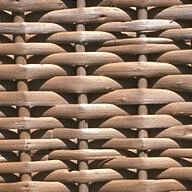
\includegraphics[scale=0.6]{./images/textures/basket}}
   \subfigure{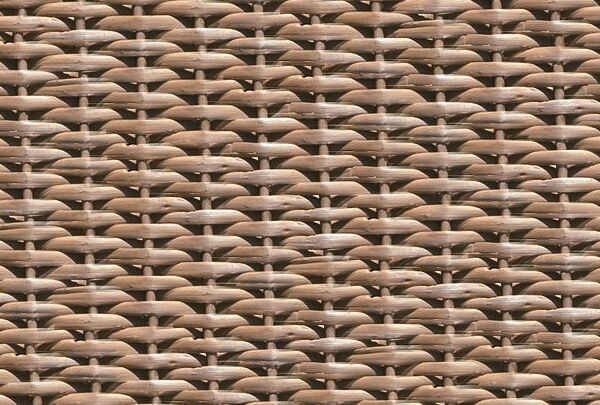
\includegraphics[scale=0.283]{./images/textures/basket_syn}}
   \caption{A regular texture which has been synthesized with minimal effort.}
   \end{center}
\end{figure}

\begin{figure}[!htbp]
   \begin{center}
   \subfigure{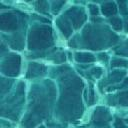
\includegraphics[scale=0.9]{./images/textures/water}}
   \subfigure{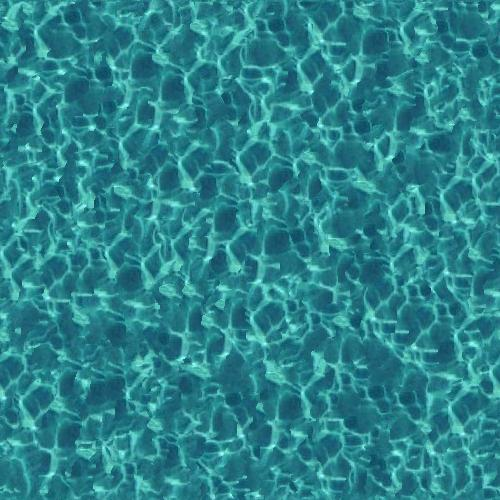
\includegraphics[scale=0.23]{./images/textures/water_syn}}
   \caption{An irregular texture which has synthesized to a larger texture using various image processing techniques.}
   \end{center}
\end{figure}

\subsection{Texture Compression Methods}
\subsubsection{Ericsson Texture Compression}
The Sony Ericsson Texture Compression algorithm, originally under the name iPACKMAN during development, targeted embedded devices such as cell phones. ETC1 uses a four-by-four block of pixels to create the compressed 64-bit output. The block is then divided into either a four-by-two or a two-by-four block. A base color is then stored for each divided block, using four bits for each channel, which becomes RGB444. The remaining 20 bits for each divided block are used to store the modulation of luminance for each pixel. ETC1 is better suited for mobile devices and is supported under Android 2.2.

ETC2 is currently under development and is to be backward compatible with ETC1 and will be able to compress texture data that contains an alpha channel. \citep{Strom2005}

\begin{figure}[!htbp]
\begin{center}
\subfigure{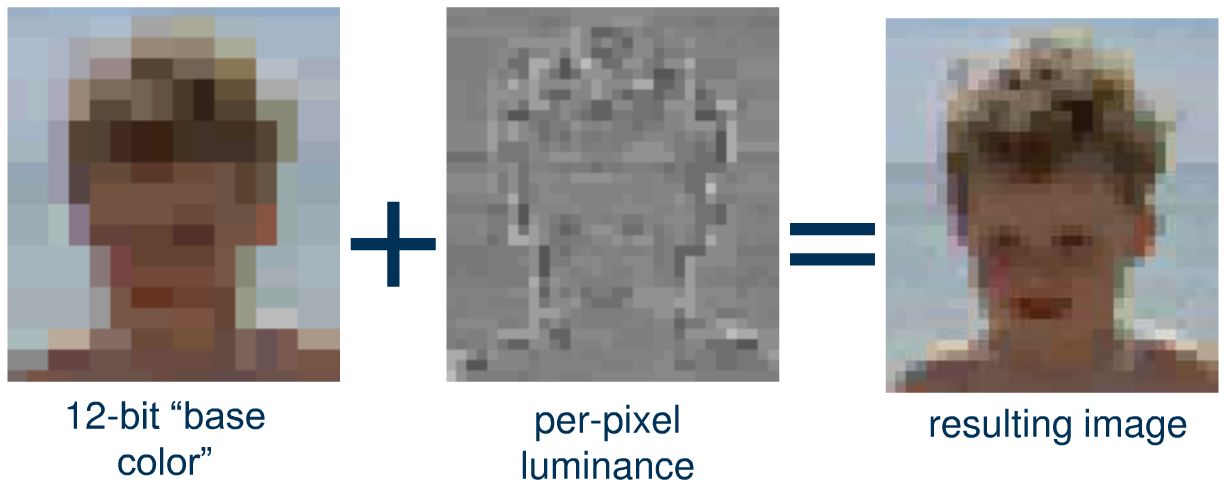
\includegraphics[scale=0.35]{./images/textures/ipackman}}
\caption{The base colors are shown for each block on the left image, while luminance modulation is shown in the middle. The final image is the decompressed image.}
\end{center}
\end{figure}

\subsubsection{S3TC (DXT1-DXT5)}
S3TC was developed by S3 Graphics and was improved over several iterations to compress textures that typically have already been arranged into larger texture atlases. S3TC has the ability to compress textures at a 1 to 6 ratio for textures without alpha information, and 1 to 4 for textures that do contain alpha information.

DXT1 uses 16 input pixels and will output 64 bits of information. This consists of two 16-bit RGB555 values and a 4 by 4 lookup table.

DXT2 and DXT3 compresses data at a 1 to 4 ratio. Using 16 input pixels, it outputs 64 bits of channel data and 64 bits of color data, encoded in a similar fashion to DXT1. This method works better on gradient textures.

DXT4 and DXT5 can compress data at a 1 to 4 ratio. Using 16 input pixels, it outputs 64 bits of channel data and 64 bits of color data. This method is more suited for noisier textures. The reference data values for alpha and color data are calculated such that:
\[
if a_0 > a_1, then  {a_2 = 6a_0+1a_1\over7},{a_3 = 5a_0+2a_1\over7},... ,{a_7 = 1a_0+6a_1\over7}
\]
\[
else {a_2 = 4a_0+1a_1\over5}...{a_5 = 1a_0+4a_1\over5}
\]

S3TC has the current problem that data can be lost in the interpolation process, resulting in artifacts in the decompressed texture. These can be avoided with using the proper method with the right type and kind of texture. \citep{Iourcha1999}

\begin{figure}[!htbp]
\begin{center}
\subfigure{\includegraphics[scale=0.7]{./images/textures/Shades_red}}\\
\subfigure{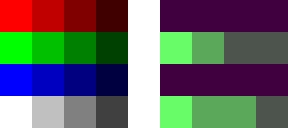
\includegraphics[scale=0.7]{./images/textures/Shades_colour}}
\end{center}
\caption{The errors for gradient textures is shown in the top set of images. The right shows the result of a reduced color palette, which cannot interpolate the original colors at all.}
\end{figure}

\clearpage
\newpage
\section{Research Goals}

The main objective is to construct a lossy method that can dither and compress images into a smaller data set that returns satisfactory results after decompression. It is expected that smaller palettes and aggressive compression will result with smaller data sets, but can also return images that have degraded in quality. The opposite is also true in that larger palettes and easier compression results in larger data sets and higher quality images. The final goal is to find a compromise between these two algorithms.

This is will be achieved by first dithering an image, and then performing various methods to further compress the resulting data. This will include DXT compression and a self made algorithm that saves the difference between a source pixel and neighboring pixels.

\subsection{Convert Images to PPM}
The first objective is to convert test data into PPM format. Most of the images available from standard test image databases are in the TIFF or BMP format. These can easy converted by using the open source program Irfanview with the following command:

\begin{center}
\begin{figure}[!htbp]
\begin{verbatim}
$ convert image.tiff image.ppm
\end{verbatim}
\end{figure}
\end{center}

This will result in a PPM file that contains the header, height, width and number of colors per channel. The remaining data is a raster of height rows from top to bottom containing a triplet of red, green and blue values.

\begin{figure}[!htbp]
\begin{center}
\subfigure{\includegraphics[scale=0.3]{./images/test_images/lena}}
\subfigure{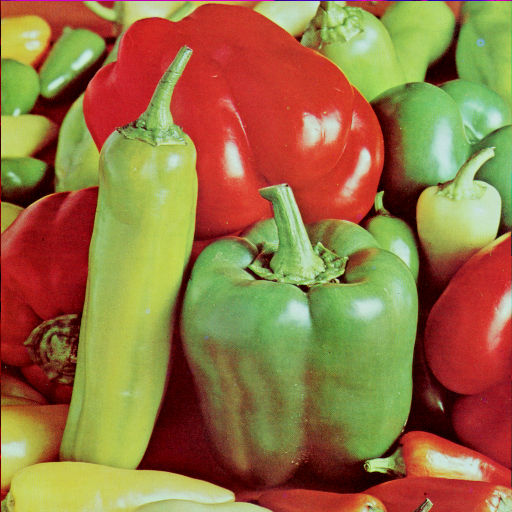
\includegraphics[scale=0.3]{./images/test_images/peppers}}
\end{center}
\caption{Examples of regular images from the USC-SIPI Database.}
\end{figure}

\subsection{Perform Dithering on Image Data}
The next step is to perform dithering on the desired images to reduce the number of colors used in each image. For the purpose of this research, Ordered (Bayer) Dithering, Floyd-Steinberg Dithering, and Jarvis, Judice, and Ninke  (JJN) Dithering were implemented. A fourth method I created will also be applied in this step, allowing the resulting image to be compared with published algorithms.

\subsection{Perform Compression on Undithered Images}
The same images will be compressed without performing dithering beforehand.

\subsection{Perform Compression on Dithered Images}
The images that have been dithered will be compressed using standard techniques that allow for random access. This will include DXT, ETC, and a custom compression method.

\subsection{Analyze and Compare Results}
As images are manipulated using dithering and compression, statistics are collected that will allow for quantitative and qualitative analysis. Using these, a decision can be made on which methods are more effective in returning images with fewer artifacts and noise.

\subsection{Graphical User Interface}
To view the results of using the above methods, a Graphical User Interface (GUI) will be developed. In the GUI, options will be available for dithering and compression methods. For dithering, Floyd-Steinbeg, Bayer (Ordered), and Jarvis-Judice-Ninke (JJN) will be available. For compression, DXT5 and ETC will be available.

The GUI will also allow the user to load files that are in the PPM format, perform any modifications to the image, and export the final decompressed image in the original PPM format.

\newpage
\section{Methodology}
\subsection{Representing an Image}
The image data in a PPM file is represented with sets of RGB tuples that start with the upper left corner of the image, which is represented as coordinate (0,0) and proceeds in a left to right fashion as the file is read, each row being M units long and a column being N units high. The end of the file corresponds with the bottom right corner of the image to be represented as (M,N).

\subsection{Applying Dithering to an Image}
\subsubsection{Ordered Dithering}
Ordered dithering adds a specified amount of error given the location of single pixel.

\subsubsection{Error Diffusion Dithering}
Error diffusion works with a palette and finds the closest match to the pixel it is working with. This can be found by calculating the distance of the colors when placed on the color cube. The difference between the original and the substituted pixel is then used to calculate the amount of error that should be pushed to designated neighboring pixels based on the method used.

\subsection{Converting PPM to TGA}
DXT requires that files be in the TGA (Truevision Graphics Adapter) file format. PPM is used as the resulting file format after performing dithering. These can easily be converted using Irfanview or any software that supports the TGA file format.

\begin{center}
\begin{figure}[!htbp]
\begin{verbatim}
$ i_view32.exe image.ppm /convert=image.tga
$ i_view32.exe image.tga /convert=image.ppm
\end{verbatim}
\caption{The command to convert a ppm formatted image to tga, and vice versa.}
\end{figure}
\end{center}

\subsection{Applying Compression to An Image}
\subsubsection{Using DXT}
Java allows for the use of external tools through proper system calls. Using the Process Class, Java can call an external tool and provide the desired input and output parameters. The resulting file type from this process is in DDS format.

\begin{center}
\begin{figure}[!htbp]
\begin{verbatim}
Process p = new ProcessBuilder( "crunch.exe", "-file", filein,
                                               "/out", fileout );
\end{verbatim}
\end{figure}
\end{center}

While the process is running, a buffer is created that can get full and cause the program to block until the buffer is cleared. This is easily accomplished by providing a file for the buffer to output to directly.

\begin{center}
\begin{figure}[!htbp]
\begin{verbatim}
p.redirectOutput(new File("output.txt"));
\end{verbatim}
\end{figure}
\end{center}

\subsubsection{Using ETC}
Java allows for the use of external tools through proper system calls. Using the Process Class, Java can call an external tool and provide the desired input and output parameters. The resulting file type from this process is in DDS format.

\begin{center}
\begin{figure}[!htbp]
\begin{verbatim}
Process p = new ProcessBuilder("etcpack.exe", input, output);
\end{verbatim}
\end{figure}
\end{center}

While the process is running, a buffer is created that can get full and cause the program to block until the buffer is cleared. This is easily accomplished by providing a file for the buffer to output to directly.

\begin{center}
\begin{figure}[!htbp]
\begin{verbatim}
p.redirectOutput(new File("output.txt"));
\end{verbatim}
\end{figure}
\end{center}

\subsubsection{Using the Proposed Method}
After dithering an image, each pixel can be represented as a single 8-bit entity. Using this information, a single pixel can be stored with increased accuracy while, neighboring pixels can be stored using fewer bits. Using a fixed number of bits, random access of a block of pixels is possible without having to decode the entire image.

\begin{figure}[!htbp]
\begin{center}
\subfigure{\includegraphics[scale=0.4]{./images/output_images/lena}}
\subfigure{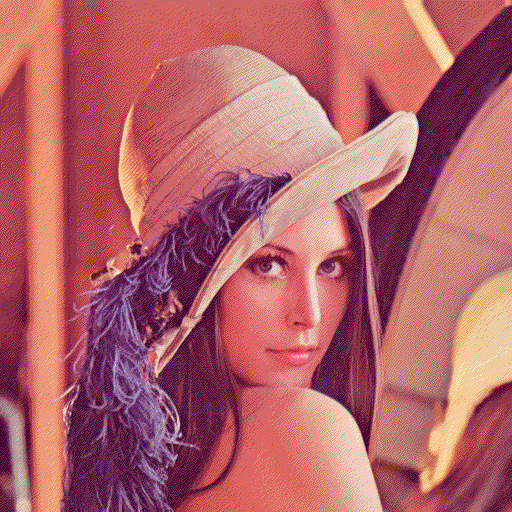
\includegraphics[scale=0.4]{./images/output_images/dith_lena}}
\caption{Left: Original image. Right: Dithered Image.}
\end{center}
\end{figure}


\begin{figure}[!htbp]
\begin{center}
\subfigure{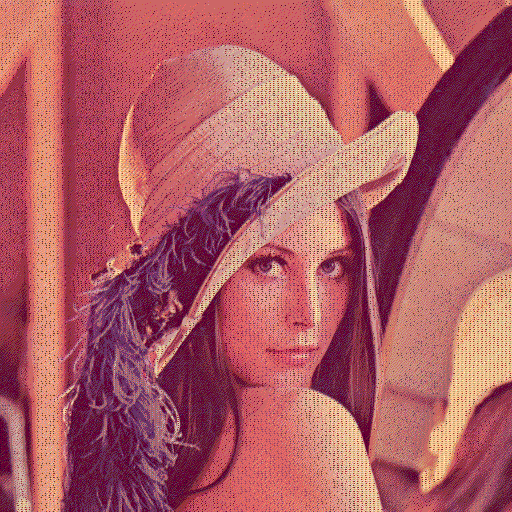
\includegraphics[scale=0.4]{./images/output_images/temp}}
\caption{The final decompressed image.}
\end{center}
\end{figure}

\subsection{Tools}
Various tools will be used to perform the proposed method. All images will be viewed using GIMP. The algorithms will be written from scratch as needed using the Java 7 JDK environment. Any quantitative data extracted will be stored in basic CSV file and images will be converted to PPM format to collect metrics.

\subsection{Evaluation}
\subsubsection{Comparing Quantitative Results}
The algorithm will be timed once the compression method has started to avoid overhead of reading the file and setting up various processes.

The primary methods of comparing original data to output data is Mean Square Error (MSE) and the Peak Signal to Noise Ratio (PSNR).

\[
MSE = \frac{1}{MN}\sum_{y=1}^{M}\sum_{x=1}^{N}[I(x,y)-I'(x,y)]^2
\]
\[
PSNR = 20*log_{10}(255/\sqrt{MSE})
\]

\subsubsection{Comparing Qualitative Results}
The results can be evaluated visually without any use of calculating actual error that the method generates. The criteria will be based on the presence of color banding, artifacts or visible blocking, and loss of detail.

\begin{figure}[!htbp]
\begin{center}
\subfigure{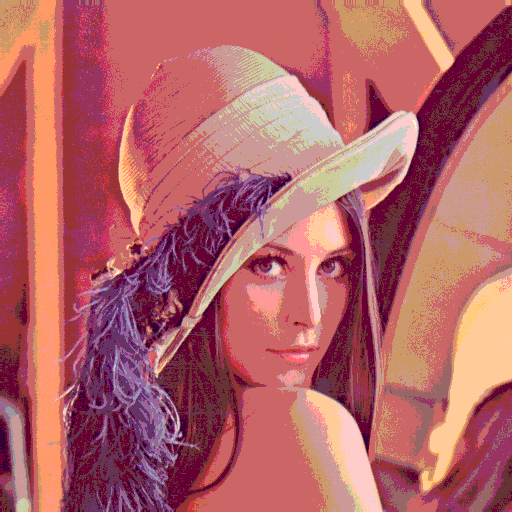
\includegraphics[scale=0.3]{./images/misc/banding}}
\subfigure{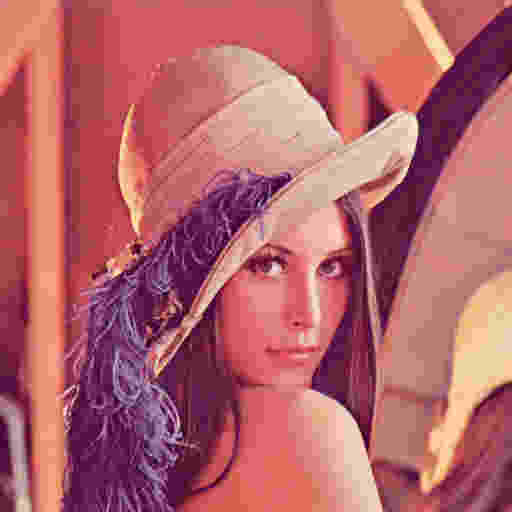
\includegraphics[scale=0.3]{./images/misc/artifacts}}
\end{center}
\caption{Left: Image banding. Right: Artifacts in the form of blocking.}
\end{figure}

\newpage
\section{Results}
\subsection{Observations}

\subsubsection{Dithering}
The new dither method, relevance, performs on par with Floyd-Steinberg dithering. Of course in some cases it does better or worse than Floyd-Steinberg, depending on the image and the palette that was specified.

\subsubsection{Compression}
The new methods Relevance 1 and 2, are quicker to compress files compared to the DirectX method, while also providing a smaller file size. Decompressing the files unfortunately resulted in images with noise and worse SNR and RMS ratios. The time constraint was achieved in such that the decompression method was faster than the compression method.

\subsubsection{Suggestions for Improvement}
When using indexed colors, a single number is used to represent a single color. Instead of indexing a single color, and tile of two by two with four potential colors can be represented instead. As blocks are traversed, tiles can be created that represent the most common patterns, and blocks are then matched to the closest tile that is available. This can also eliminate the need for a pre-specified palette if so desired when used without dithering. Using method this also increases the amount of time it takes to compress a file, as the most suitable tile must be either found or created. 

\newpage

\subsection{Statistics}
\subsubsection{Test Images}
\begin{figure}[!htbp]
\begin{center}
\subfigure{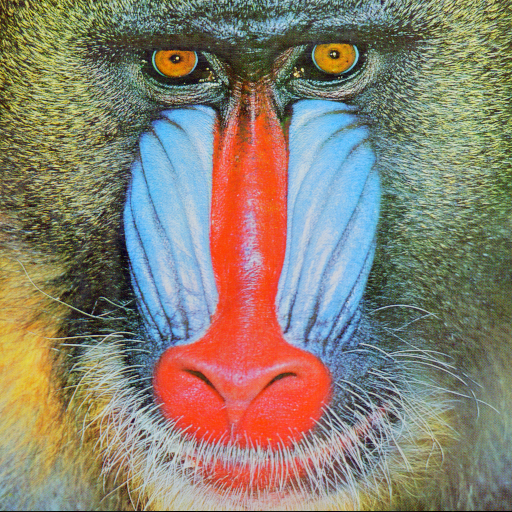
\includegraphics[scale=0.25]{./images/test_images/baboon}}
\subfigure{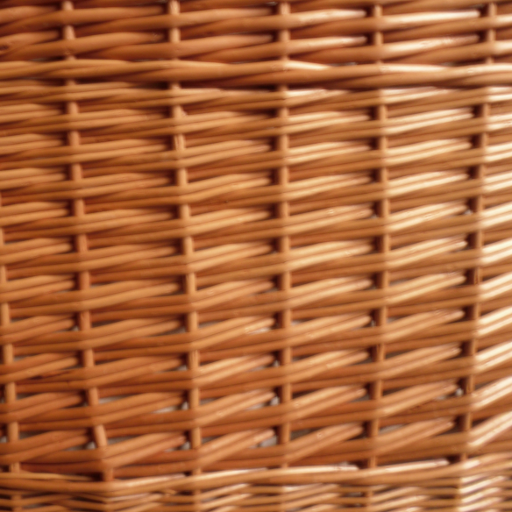
\includegraphics[scale=0.25]{./images/test_images/bamboo}}
\subfigure{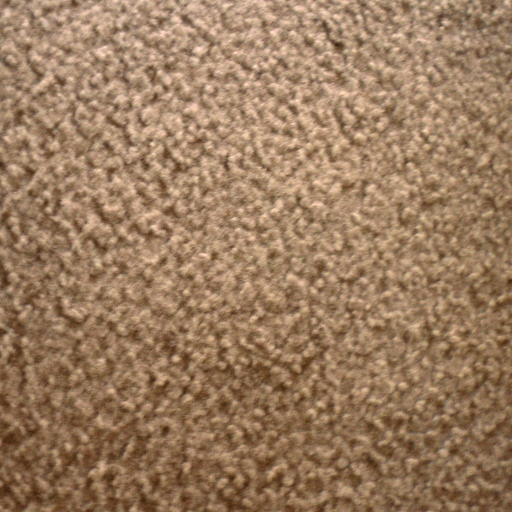
\includegraphics[scale=0.25]{./images/test_images/carpet}}
\subfigure{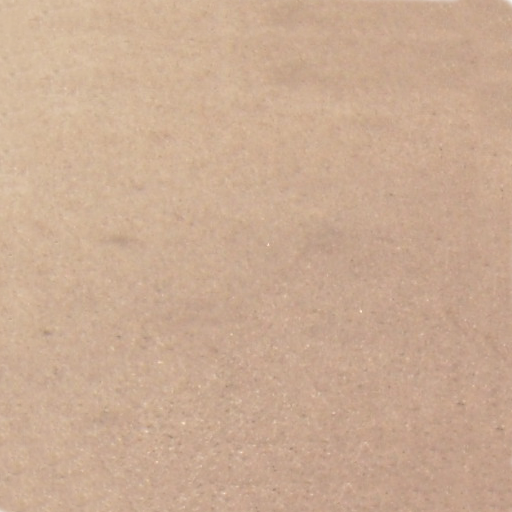
\includegraphics[scale=0.25]{./images/test_images/concrete}}
\subfigure{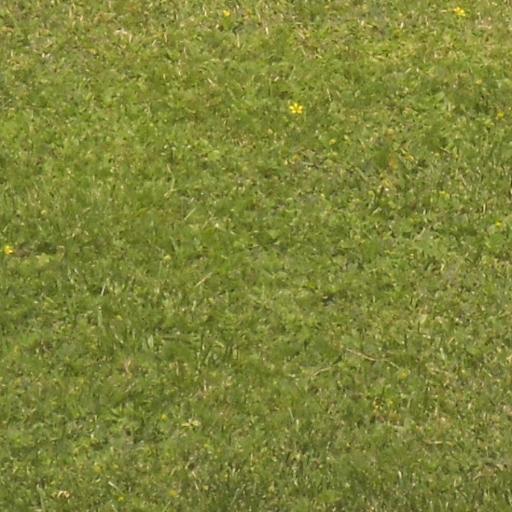
\includegraphics[scale=0.25]{./images/test_images/grass}}
\subfigure{\includegraphics[scale=0.25]{./images/test_images/lena}}
\subfigure{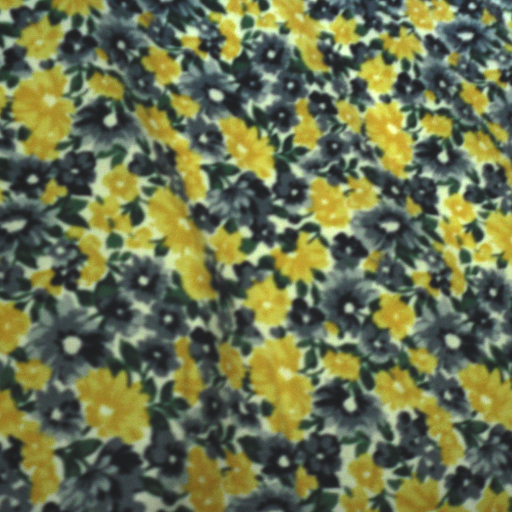
\includegraphics[scale=0.25]{./images/test_images/pattern}}
\subfigure{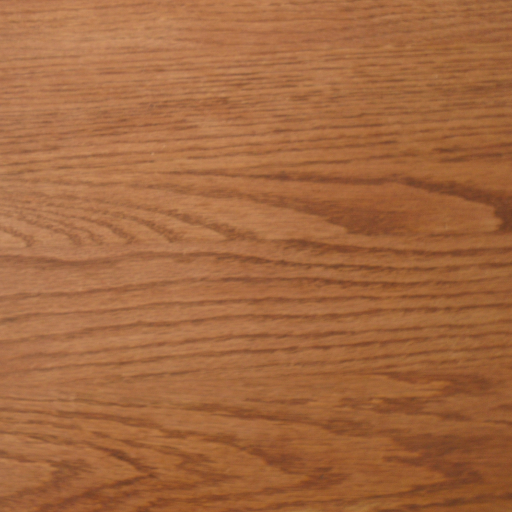
\includegraphics[scale=0.25]{./images/test_images/wood}}
\end{center}
\caption{The set of test images used. In order: Baboon, Bamboo, Carpet, Concrete, Grass, Lena, Pattern, Wood.}
\end{figure}

\newpage

\captionsetup{width=7in}

\renewcommand{\arraystretch}{.8}
\setlength{\tabcolsep}{4pt}
\subsubsection{Control Methods}
\begin{center}
\begin{longtable}{| l | l | l | l | l | l | l |}

\caption{Statistics for Compressed Images without Dithering} \\
\hline
Compression & Time & Ratio & Decompression & Time & RMS & SNR \\
\hline
\endfirsthead
\caption[]{Statistics for Compressed Images without Dithering}  \\
\hline
Compression & Time & Ratio & Decompression & Time & RMS & SNR \\
\hline
\endhead

\multicolumn{7}{ |c| }{Baboon} \\ \hline
\input{undithered.out}
\end{longtable}
\end{center}

\newpage
\subsubsection{Dither Methods}
\begin{center}
\begin{longtable}{| l | l | l | l | l |}

\caption{Statistics for Dithered Images} \\
\hline
\# of Colors & Dither & Time & RMS & SNR \\
\hline
\endfirsthead
\caption[]{Statistics for Dithered Images}  \\
\hline
\# of Colors & Dither & Time & RMS & SNR \\
\hline
\endhead

\multicolumn{5}{ |c| }{Baboon} \\ \hline
\input{dither.out}
\end{longtable}
\end{center}

\newpage
\subsubsection{Compression Methods}
\begin{center}
\begin{longtable}{| l | l | l | l | l |}

\caption{Statistics for Compressed Images with Dithering} \\
\hline
\# of Colors & Dither & Compression & Time & Ratio \\
\hline
\endfirsthead
\caption[]{Statistics for Compressed Images with Dithering}  \\
\hline
\# of Colors & Dither & Compression & Time & Ratio \\
\hline
\endhead

\multicolumn{5}{ |c| }{Baboon} \\ \hline
\input{compress.out}
\end{longtable}
\end{center}

\newpage
\subsubsection{Decompression Methods}
\begin{center}
\begin{longtable}{| l | l | l | l | l | l |}

\caption{Statistics for Decompressed Images with Dithering} \\
\hline
\# of Colors & Dither & Decompression & Time & RMS & SNR \\
\hline
\endfirsthead
\caption[]{Statistics for Decompressed Images with Dithering}  \\
\hline
\# of Colors & Dither & Decompression & Time & RMS & SNR \\
\hline
\endhead

\multicolumn{6}{ |c| }{Baboon} \\ \hline
\input{decompress.out}
\end{longtable}
\end{center}

\clearpage
\hyphenpenalty=5000
\tolerance=1000
\bibliography{bibfile}

\end{document}
